\section{Description des différentes spécifications définies en travaux dirigés}

\subsection*{Objectif}

Les spécifications ont pour objectif de définir le comportement attendu du système, c’est-à-dire 
\textbf{ce que le circuit doit faire} en réponse au cahier des charges. 
Elles constituent une description \textbf{fonctionnelle} du système, exprimée du point de vue de son 
\textbf{environnement} — c’est-à-dire de tout ce qui interagit avec lui, sans se soucier de son 
implémentation interne.

\medskip

Cette phase correspond au \textbf{niveau de spécification fonctionnelle} dans le diagramme en Y. 
Elle adopte une approche \textbf{boîte noire}, centrée sur les entrées et sorties observables, 
indépendamment de toute considération technologique (langage, type logique, fréquence, etc.).

\medskip

Le cahier des charges indique que le circuit doit pouvoir \textbf{communiquer à la fois avec le système 
de trame LIN et avec un microcontrôleur}. 
Afin de clarifier les fonctions du système, nous avons choisi de le \textbf{décomposer en deux sous-blocs principaux} :
\begin{itemize}
    \item un bloc de \textbf{réception de trame LIN}, chargé de décoder et de stocker les données reçues ;
    \item un bloc d’\textbf{interface microprocesseur}, permettant l’échange de données et de signaux de contrôle avec le microcontrôleur.
\end{itemize}

\begin{figure}[H]
   \centering
   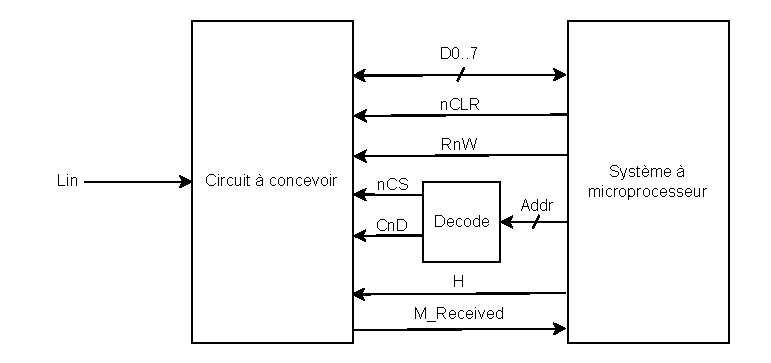
\includegraphics[width=0.8\linewidth]{images/CDC/Schema_cdc_final.pdf}
   \caption{Description fonctionnelle du circuit à concevoir}
   \label{fig:placeholder}
\end{figure}

\subsection{Interface Microprocesseur}

Ce sous-système permet la communication entre le circuit et le microprocesseur.  
Les signaux décrits ici représentent les \textbf{flux d’informations échangés} (données, commandes, synchronisation, validation), 
sans spécifier leur codage logique ni leur type de signal électrique.

\begin{center}
\renewcommand{\arraystretch}{1.2}
\small
\begin{tabularx}{\textwidth}{|c||c|c|X|}
    \hline			
    \textbf{Signal} & \textbf{Sens} & \textbf{Nature} & \textbf{Rôle fonctionnel}  \\ \hline 
    D\_BUS & Bidirectionnel & Données & Bus de transfert de données entre le microprocesseur et le circuit \\ 
    CS & Entrée & Commande & Sélection du circuit (validation de la communication) \\ 
    RW & Entrée & Commande & Indique une opération de lecture ou d’écriture \\ 
    CD & Entrée & Commande & Sélectionne entre registre de commande et registre de données \\ 
    RESET & Entrée & Commande & Réinitialisation du système \\ 
    MSG\_RECEIVED & Sortie & Indicateur & Signal indiquant la fin de réception d’une trame \\ 
    CLK & Entrée & Synchronisation & Signal d’horloge du système \\ 
    \hline  
\end{tabularx}
\end{center}

\subsection{Bloc Réception de Trame LIN}

Ce bloc assure le \textbf{décodage séquentiel} des trames LIN reçues.  
Il analyse le flux série provenant du bus LIN et extrait les octets de données en respectant la structure du protocole.

\begin{center}
\renewcommand{\arraystretch}{1.2}
\small
\begin{tabularx}{\textwidth}{|c||c|c|X|}
    \hline			
    \textbf{Signal} & \textbf{Sens} & \textbf{Nature} & \textbf{Rôle fonctionnel}  \\ \hline 
    LIN\_RX & Entrée & Données & Flux série reçu depuis le bus LIN \\ 
    DATA\_OUT & Sortie & Données & Octet de données extrait et validé \\ 
    VALID & Sortie & Indicateur & Indique la disponibilité d’un nouvel octet reçu \\ 
    \hline  
\end{tabularx}
\end{center}

\subsection{Mémoire FIFO}

Ce bloc a pour rôle de \textbf{stocker temporairement les octets reçus} avant leur transfert vers le microprocesseur.  
Il fonctionne selon le principe « premier entré, premier sorti ».

\begin{center}
\renewcommand{\arraystretch}{1.2}
\small
\begin{tabularx}{\textwidth}{|c||c|c|X|}
    \hline
    \textbf{Signal} & \textbf{Sens} & \textbf{Nature} & \textbf{Rôle fonctionnel} \\ \hline
    DATA\_IN & Entrée & Données & Octet à mémoriser dans la file FIFO \\ 
    DATA\_OUT & Sortie & Données & Octet extrait de la file FIFO \\ 
    WRITE\_REQ & Entrée & Commande & Requête d’écriture (nouvelle donnée reçue) \\ 
    READ\_REQ & Entrée & Commande & Requête de lecture (demande du microprocesseur) \\ 
    EMPTY & Sortie & Indicateur & Indique que la FIFO est vide \\ 
    FULL & Sortie & Indicateur & Indique que la FIFO est pleine \\ 
    \hline
\end{tabularx}
\end{center}

\subsection{Registre d’État}

Le registre d’état fournit une \textbf{synthèse du déroulement de la réception}.  
Il conserve les informations nécessaires à la supervision ou au diagnostic 
(erreurs détectées, nombre d’octets reçus, trame complète, etc.).

\begin{center}
\renewcommand{\arraystretch}{1.2}
\small
\begin{tabularx}{\textwidth}{|c||c|c|X|}
    \hline			
    \textbf{Signal} & \textbf{Sens} & \textbf{Nature} & \textbf{Rôle fonctionnel}  \\ \hline 
    ERR\_START & Entrée & Indicateur & Erreur sur le bit de début de trame \\ 
    ERR\_STOP & Entrée & Indicateur & Erreur sur le bit de fin de trame \\ 
    ERR\_SYNC & Entrée & Indicateur & Erreur de synchronisation \\ 
    BYTE\_COUNT & Entrée & Données & Nombre d’octets reçus dans la trame \\ 
    FRAME\_VALID & Entrée & Indicateur & Validation de la réception complète \\ 
    STATE\_OUT & Sortie & Données & Octet d’état global de la réception \\ 
    \hline  
\end{tabularx}
\end{center}
